% Diapo d'intro

\frame{\frametitle{\textbf{MeForBio} (IRCCyN team, ECN): Formal Methods for Bioinformatics}

\begin{block}{Research axes}
\begin{itemize}
\item Models: automata, Petri nets, boolean networks, process algebra ($\rightarrow$~process hitting)
\item Extended with: time (\textbf{chronometry} vs \textbf{chronology}) and/or parameters
\item Analysis techniques: \textbf{model-checking}, \textbf{control}, \textbf{abstraction}, \textbf{parameters inference}
\item Applied (and/or designed) to biology, e.g. biological regulatory networks
\end{itemize}
\end{block}

}

\begin{frame}[c]
  \frametitle{\textbf{MeForBio} (IRCCyN team, ECN)}

%\textbf{MeForBio} (IRCCyN team, ECN): Formal Methods for Bioinformatics

\bigskip\footnotesize
\begin{tabular}{ccc}
  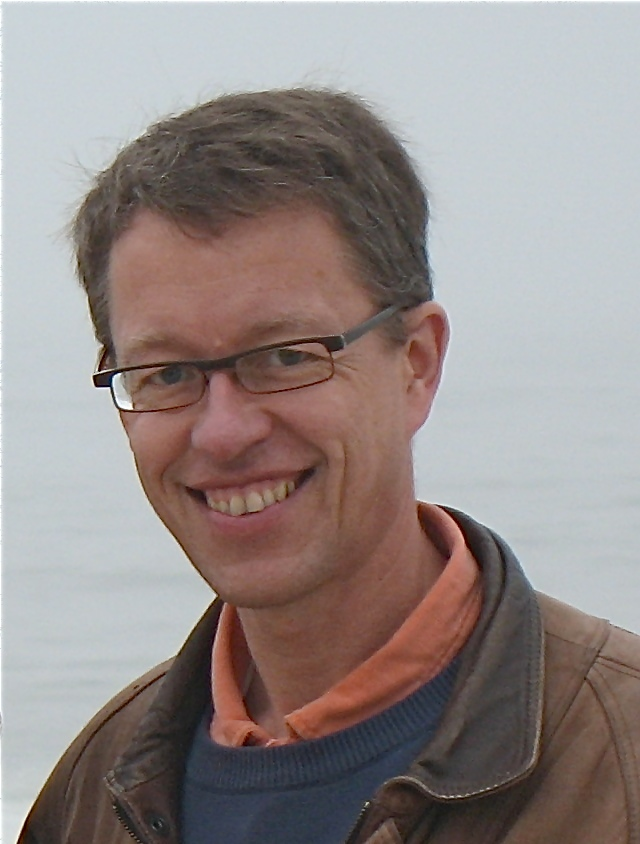
\includegraphics[height=1.5cm]{figures/Olivier.jpg}
& 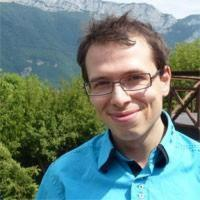
\includegraphics[height=1.5cm]{figures/Morgan.jpg}
& 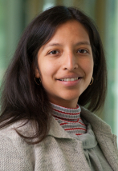
\includegraphics[height=1.5cm]{figures/Carito.jpg} \\
  \tval{Olivier ROUX} & \tval{Morgan MAGNIN} & \tval{Carito GUZIOLOWSKI} \\
  Professor \& team leader & Associate professor & Associate professor \\&&\\
  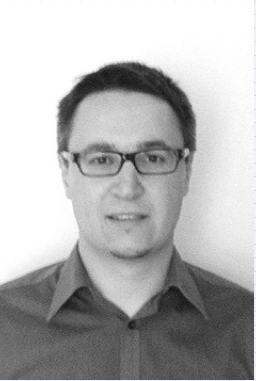
\includegraphics[height=1.5cm]{figures/Julien.jpg}
& 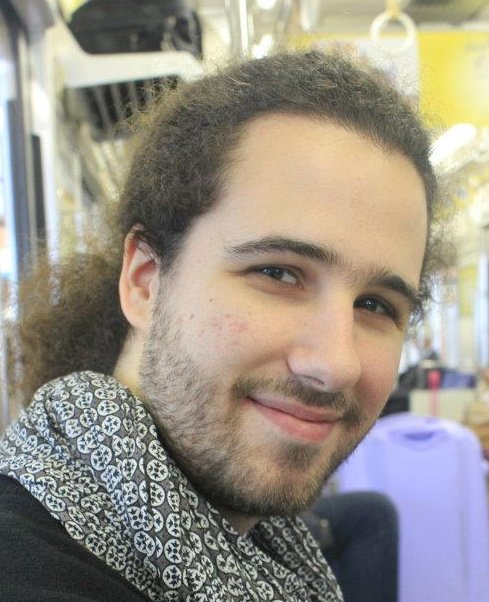
\includegraphics[height=1.5cm]{figures/Maxime.jpg}
& 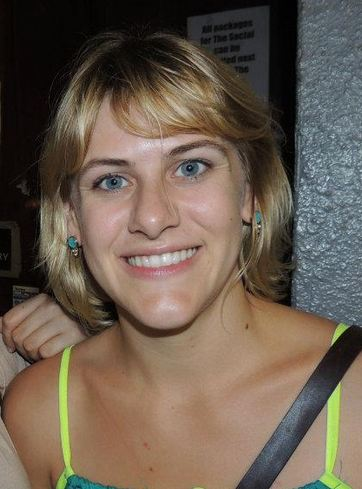
\includegraphics[height=1.5cm]{figures/Courtney.jpg} \\
  \tval{Julien GRAS} & \tval{Maxime FOLSCHETTE} & \tval{Courtney CHANCELLOR} \\
  Research engineer & 3\textsuperscript{rd} year PhD student & 2\textsuperscript{nd} year PhD student \\    
\end{tabular}
\end{frame}


\frame{\frametitle{Today's issue}

\begin{alertblock}{Tricky question}
How can we study complex dynamical biological systems, \textbf{involving up to 1.000 interacting components}?
%\begin{center}
%  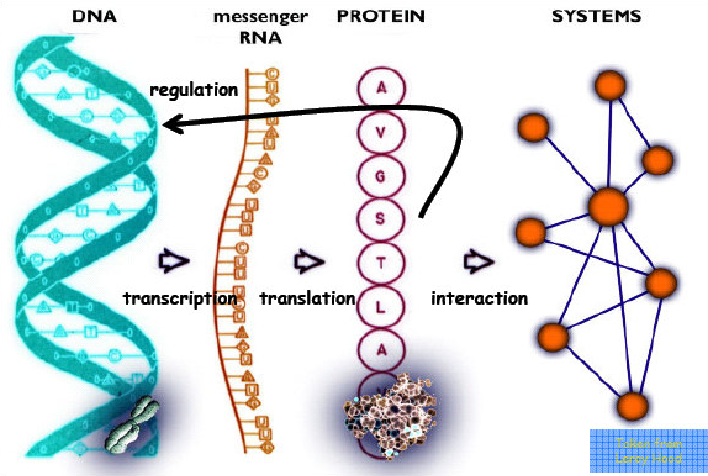
\includegraphics[height=2cm]{figures/dnascheme_white.png}
%\end{center}
\end{alertblock}

\begin{block}{Observation}
\begin{itemize}
\item Classical model-checking approaches suffer from state space explosion
\item Leads:
\begin{itemize}
\item Taking profit for Process Algebra structure, based on a \textbf{compact representation of the interactions} 
\item Develop \textbf{static analysis approaches} to verify some crucial properties, e.g. stable states, reachability, key processes, $\ldots$
\end{itemize}
\end{itemize}
\end{block}

}


\frame{\frametitle{Contribution}

\begin{alertblock}{Scientific challenge}
How can we cope with the analysis of \textbf{large-scale systems}, involving up to 1.000 interacting components?
\end{alertblock}

\begin{block}{Objectives of this talk (and Lo�c's one)}
\begin{itemize}
\item Introduce a Process Algebra inspired framework based on a compact representation of the interactions
\item Develop efficient \textbf{static analysis approaches} to answer most common problems 
\item Apply the methodology to large-scale biological regulatory networks 
\end{itemize}
\end{block}

%\begin{block}{Joint work with}
%\begin{itemize}
%\item K. Inoue (NII) 
%\item L. Paulev� (LRI)
%\item O. Roux (IRCCyN) 
%\end{itemize}
%\end{block}

}

